\section{Knowledge graph}
\label{section: knowledge_graph}
Transitions in the HGraph are executed and reviewed, the KGraph then act as memory to store the reviewed transitions using a $success factor$. The success factor describes how transitions in the past have been executed, a high success factor means coming up high in the list of action recommendations. \\

\subsection{Definition}
A knowledge graph contains information about objects. $ObjectSetNodes$ describe the objects knowledge is known about, and transitions from $objectSetNodes$ point to $changeOfConfSetNodes$ indicating which part of the configuration was changed. The transition describes in detail how the objects in the object set can change their configuration set.\\ 

Formally, a \textbf{knowledge graph}, $G^{knowledge} = (V, E)$ comprising $V = \{V^{ob}_{i}, V^{\Delta conf}_{j}\}$, $E \in \{\tau_{(i,j)}| V_i\in V^{ob}_{i}, V_j \in V^{\Delta conf}_{j}\}$ where $i$ and $j$ are unique identifiers.\\

\paragraph{Reviewing an Executed Transaction}
Controllers and system models which produce desirable results (low prediction errors, many successfully executed transitions) should be used over controllers producing less desirable results. To keep track of how 'good' a transition was, feedback on a transition is introduced. Feedback consists of 2 parts, a transition succeeding or failing and the average prediction error. Feedback is stored, and converted to a success factor $\alpha \in [0.1, 1]$. Testing and fine-tuning $\alpha$ has not yet occurred, thus the following equation for the success factor has to be taken with a grain of salt. 
\begin{equation}
\alpha = 
      \begin{cases}
        (0.5 - \epsilon_{avg})^{1-\frac{success}{success + fails}}       & \text{if $\epsilon_{avg} < 0.4$}\\
      0.1^{1-\frac{success}{success + fails}}       & \text{if $\epsilon_{avg} \geq 0.4$}\\
    \end{cases}    
    \label{equation: success_factor}
\end{equation}

Where $\epsilon_{avg}$ is the average prediction error over all stored prediction errors, $success$ is the number of times a transition was successfully executed and $fails$ is the number of times a transition failed. \\

\paragraph{Knowledge Graph Flowchart}
Let's walk through the KGraphs flowchart displayed in \cref{figure: flowchart_kgraph}. Incoming action feedback (success/failure and average prediction error of an executed transition) is checked against existing knowledge in the KGraph and updated accordingly to \cref{equation: success_factor}. A query asking for an action suggestion is answered by an empty or ordered of action suggestions, the order is determined by the success factor. For the observant reader, there is no outgoing arrow named "environment knowledge" such as displayed in \cref{figure: block_framework}, which is left out on purpose since the ontology is not a part of the literate study. 

\newpage
\begin{figure}[H] \centering
\begin{tikzpicture}[node distance = 4.5cm]
    % Nodes
    \node [block, fill=green!50] (first) {Update existing transition with feedback};
    
    % legend 
    \node[text width=2.8cm, yshift=1cm, right of=first, text centered, rounded corners, minimum height=1em, label={[name=lab, yshift=0.4cm, left]\textbf{Legend}}, node distance=7cm] (legend1) {\small Update KGraph};
    \node[rectangle, draw, left of=legend1, fill=green!50, rounded corners, minimum height=1em, minimum width=1cm, node distance=2cm] (legend1color) {};
    \node[text width=2.8cm, below of=legend1, text centered, minimum height=1em, node distance=0.7cm] (legend2) {\small Query KGraph};
    \node[rectangle, draw, left of=legend2, fill=red!40, rounded corners, minimum height=1em, minimum width=1cm, node distance=2cm] (legend2color) {};
   
    
    % nodes, first row 
    
    \node [decision, below of=first, node distance=4.5cm, fill=red!40] (has_controller) {The ObjectSet- Node already contains outgoing transition with equal parameterisation};
    \node [block, left of=has_controller, fill=green!50] (new_transition) {Generate new transition on existing node};
    \node [block, right of=has_controller, node distance=3.8cm] (send_feedback) {Send ordered list with controllers and models};
    
    % nodes, second row 
    \node [decision, fill=red!40, below of=has_controller, node distance=4.5cm] (obj_exist) {Object already in HGraph};
    \node [decision, fill=red!40, right of=obj_exist, node distance=3.8cm] (obj_exist2) {Object in HGraph};
    \node [block, fill=green!50, left of=obj_exist] (new_object) {Generate new object + new transition with feedback};
    \node [block, right of=obj_exist2, node distance=3.5cm] (no_obj) {send empty list};
   
    % Edges
    \draw[stealth-] (obj_exist) -- node[left]{action feedback} +(0,-2.5cm);
    \draw[-stealth] (obj_exist.west) -- node[above]{no} (new_object.east);
    \draw[-stealth] (obj_exist.north) -- node[left]{yes} (has_controller.south);
    \draw[-stealth] (has_controller.north) -- node[left]{yes} (first.south);
    \draw[-stealth] (has_controller.west) -- node[above]{no} (new_transition.east);
    
    \draw[-stealth] (obj_exist2.east) -- node[above]{no} (no_obj.west);
    \draw[-] (no_obj.east) -- +(1cm, 0);
    \draw[stealth-] (obj_exist2) -- node[left]{action suggestion?} +(0,-2.5cm);
    \draw[-stealth] (obj_exist2.north) -- node[left]{yes} (send_feedback.south);
    \draw[-stealth] (send_feedback.east) -| node[at end, left]{action suggestion} +(4.5cm, -6.5cm);
\end{tikzpicture}

\caption{Flowchart displaying the knowledge graph's workflow.}
\label{figure: flowchart_kgraph} 
\end{figure}

\subsection{Example KGraph}
As a result of the example hypothesis graph displayed in \cref{figure: example_hgraph}, the following knowledge graph should emerge displayed in \cref{figure: example_kgraph}. The transition containing the \ac{EMPPI} controller can be seen connecting the red sphere and robot to the changeOfConfSetNode which indicates that the position and velocity of the red sphere can be changed. And vice versa for the \ac{MPC} controller. 

\begin{figure}[H]
    \centering
    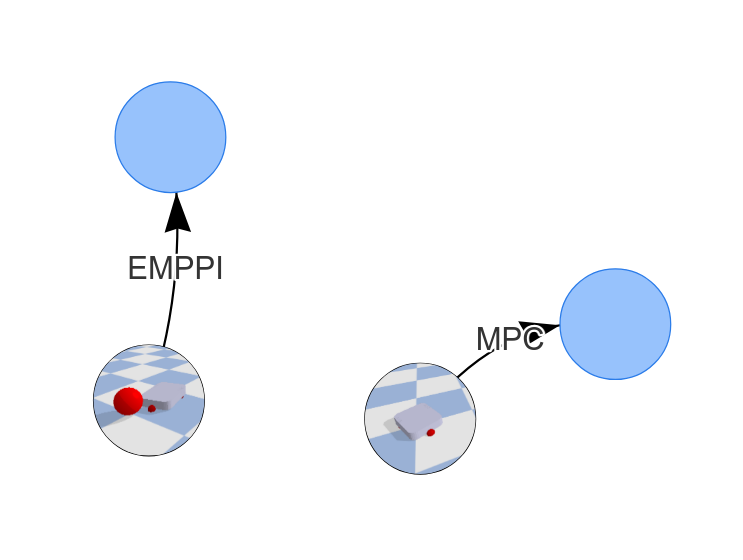
\includegraphics[width=0.6\textwidth]{figures/example_kgraph.png}
    \caption{The knowledge graph after pushing a red sphere, this knowledge graph corresponds with the hypothesis graph in \cref{figure: example_hgraph}, ChangeOfConfSetNodes are displayed in blue, objectSetNodes display an image with the objects they represent.}
    \label{figure: example_kgraph}
\end{figure}
